%************************************************
\chapter{Watch It Grow}
%************************************************

\section{Sentimental Introduction}
	Science often seems like a blackbox that relates observables. Even more often, it is rather convenient to lose touch of observables altogether, and wander in the blackbox. Performing an experiment, gets one closer to nature, to the roots of the subject.\footnote{This section can be skipped, without any loss of continuity.}

\section{The Journey}
	\subsection{Look it has begun}
		This experiment wasn't started from scratch. My guide, \myProf, had already worked with a team and created the Dipoles as described earlier. The team had also worked on the image detection algorithms, but their work wasn't usable.
		\par
		There were three tasks at hand, of which one had been significantly simplified by the prior work.
		\begin{enumerate}
			\item The Dipole
					\par
					This had one apparent problem; the dipoles had to be made virtually frictionless (which is not to say they had excessive friction, infact they would oscillate atleast about 8 times before stopping aligned with earth's magnetic field)
			\item The Image Analysis
					\par
					This part I had to start from the beginning with two basic objectives, as stated earlier; measuring the angle of the dipoles and evaluating the current to be pumped based on the temperature selected.\\
					What was known soon, was that C++ will be used for programming and linux would be the operating system, to facilitate USB interface with the AVR (next step)
			\item The Current Control Hardware
					\par
					This is simply for providing a current pulse proportional to the intensity calculated by the lattice analyser. Some schematics for this were available, but were found to be inaccurate and incomplete.
		\end{enumerate}
	
	\subsection{Time Line}
		Listed below is the event log, which has the progress as and when it was made.
		\lstinputlisting[firstline=22,title=Time Line]{../../../../README.md}
	
	\subsection{Construction of the Dipole}
		To remove the friction, there were various ideas, including use of a super conductor. However, eventually three methods were considered and experimentally tested.
		\begin{enumerate}
			\item Ferro-Fluid: 
					\par
					As it turns out, there are substances that have a ferro magnetic properties but in the liquid form. Consequently, a strong enough magnet would glide if coated with this substance.
					\par
					Experimentally, it was found that the friction was higher than the `needle on glass' setup. 
			\item Magnetic Levitation:
					\par
					A magnet can easily suspend another magnet, granted it doesn't flip. This idea was used and a magnetic cylinder was placed co-axial to the needle, using a cylindrical eraser and glue. Beneath the glass slide, an identical magnet was placed with the face that repels upwards.
					\par
					Experimentally, again it was found that the motion was more damped than the `needle on glass' setup. The reason for this case was obvious after a little analysis and closer observation. The dipole would align to the field of the magnet, viz. the magnetic field was interfering with the dipole.
			\item Air Levitation:
					This hasn't been tested yet, but the idea is to put a disc at the bottom of the needle, and pass air through it to keep it suspended.
		\end{enumerate}
	\subsection{Construction of the Lattice Analyser}
		The lattice analyser has come a long way. Image detection trials were initiated with \autoref{sampleImage}. 
		\begin{figure}[bth]
			\begin{center}
				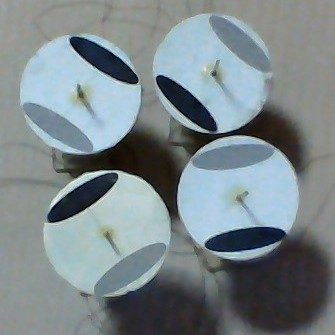
\includegraphics[width=0.7\linewidth]{../../latticeAnalyser/picture002.jpg}
			\end{center}
		\caption[Sample Image]{Sample Image}
		\label{sampleImage}
		\end{figure}

		The idea was that once the ellipses have been detected, and they are different in colour, one can evaluate from their centroids, the position and the angle of the dipole. It must be stated that earlier it was attempted to use the greyscale image as was provided. However soon the shadow interference led to using coloured patterns instead. These patterns were not printed but displayed on a screen and the camera aimed appropriately.
		\par
		So first, the algorithm for detection of relevant part of the image had to be frozen. There were two candidates for this
		\begin{enumerate}
			\item Hough Transform Method
				\par
				Either one could use the already available in OpenCV, line detection or circle detection, both would've required changing the pattern on the dipole
				\par
				Or one could use an ellipse modification for the same, which would require programming the algorithm.
			\item Contour Detection and Ellipse Fitting
				\par
				This method detects contours in a given image, and the OpenCV example also shows ellipse fitting for the same. This seemed promising too, but it seemed more expensive (computationally) than looking for predetermined shapes.
		\end{enumerate}
		This work had been done within the first few days. 
		\par

		\begin{figure}[bth]
			\begin{center}
				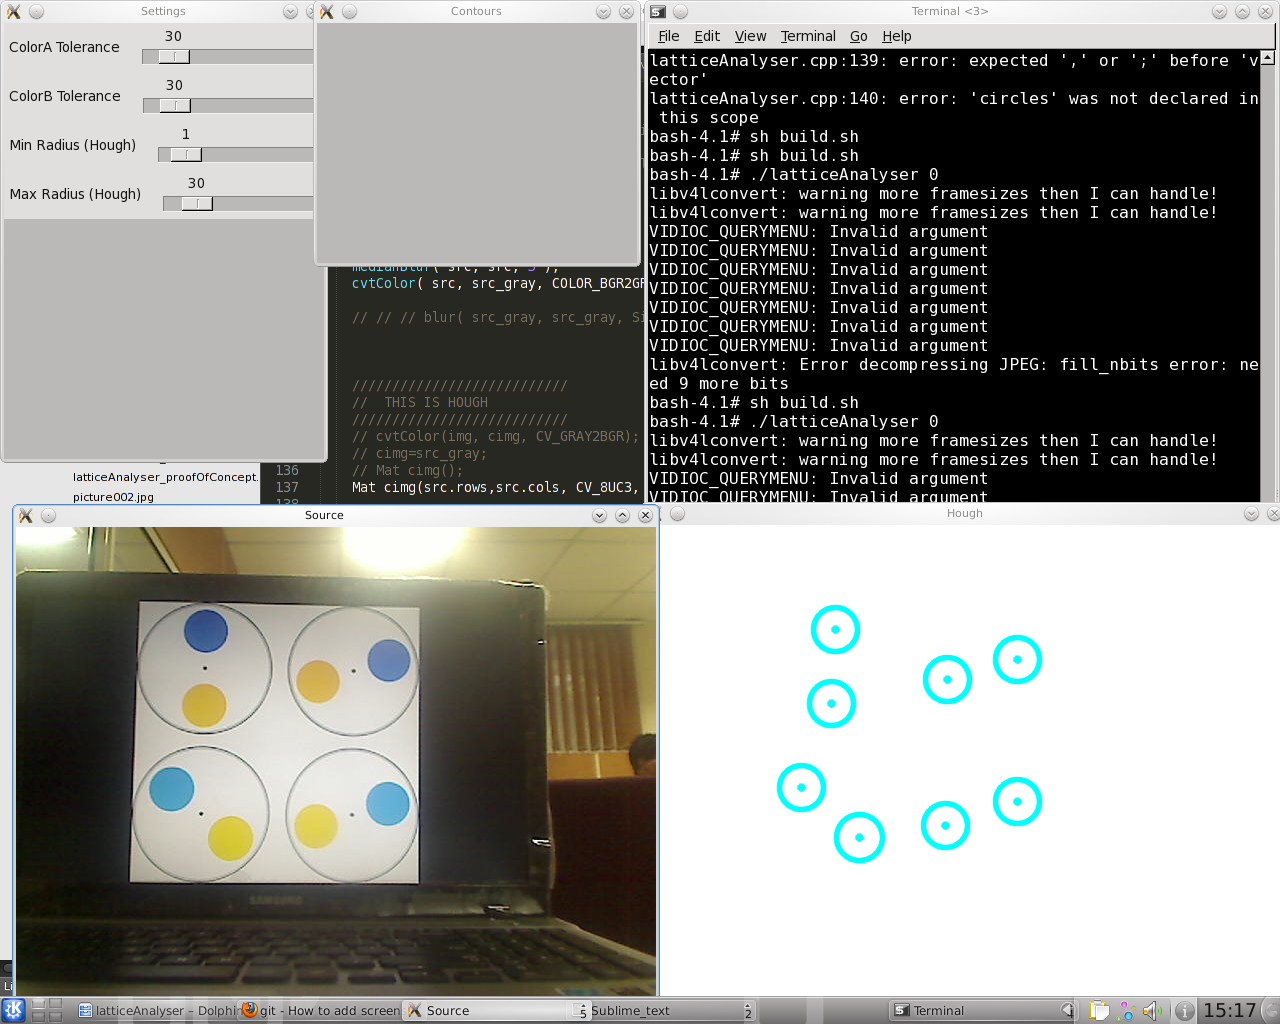
\includegraphics[width=1.1\linewidth]{../../latticeAnalyser/snapshot1.png}
			\end{center}
		\caption[Hough Transform]{Hough Transform}
		\label{snapshot1}
		\end{figure}

		\begin{figure}[bth]
			\begin{center}
				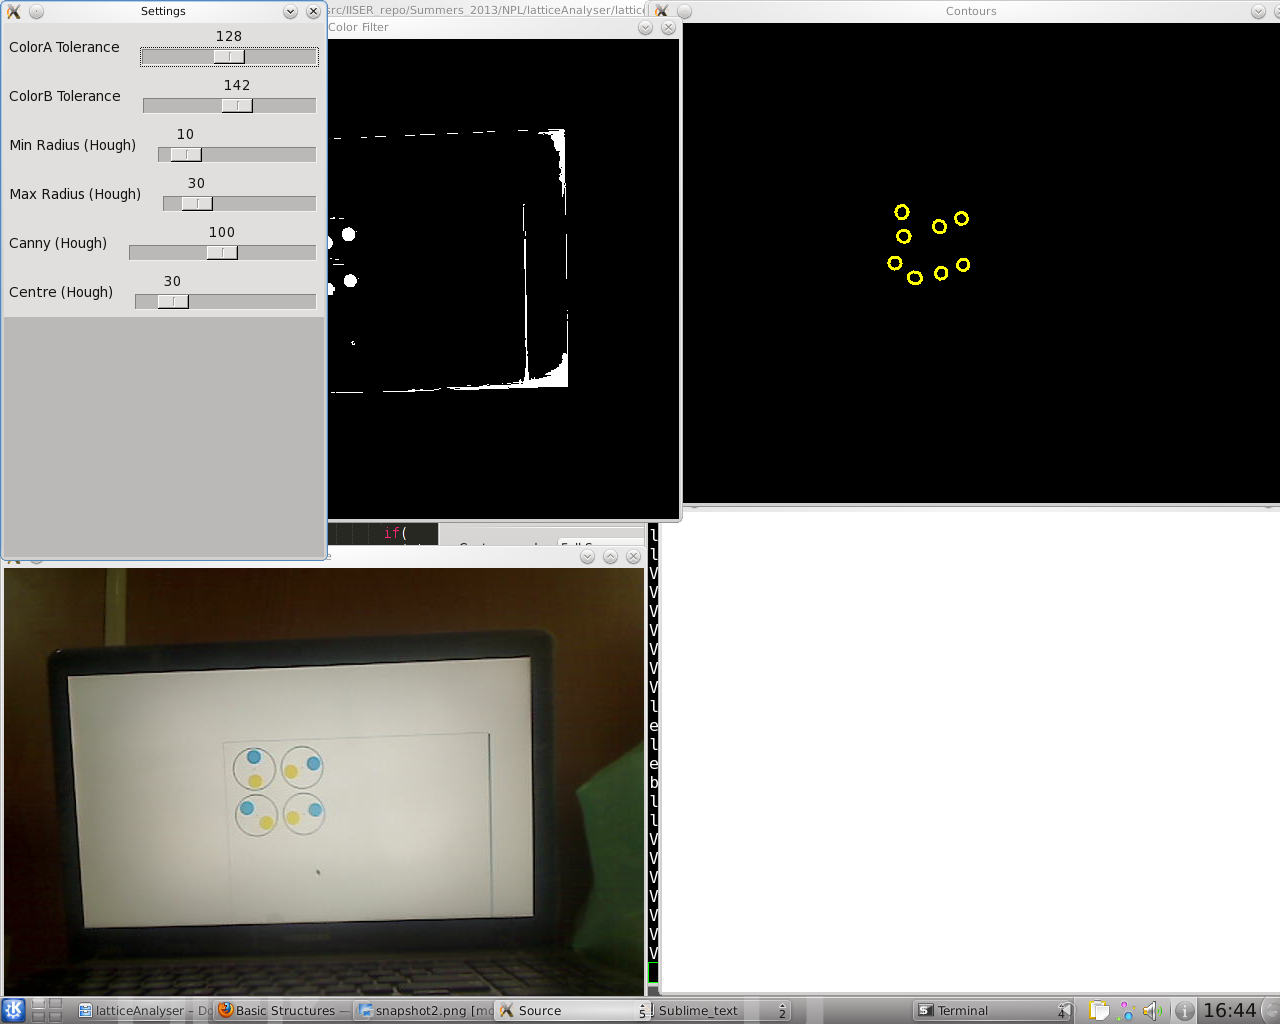
\includegraphics[width=1.1\linewidth]{../../latticeAnalyser/snapshot2.png}
			\end{center}
		\caption[Contour Detection]{Contour Detection}
		\label{snapshot2}
		\end{figure}

		Next, a colour filter was to setup to improve the accuracy. When the algorithms were implemented, it was found that the Hough Transform method often misses detection of circles, refer to \autoref{snapshot1} (this is ofcourse after attaching a video stream instead of images to the code) as compared to contour detection \autoref{snapshot2}.
		\par

		\begin{figure}[bth]
			\begin{center}
				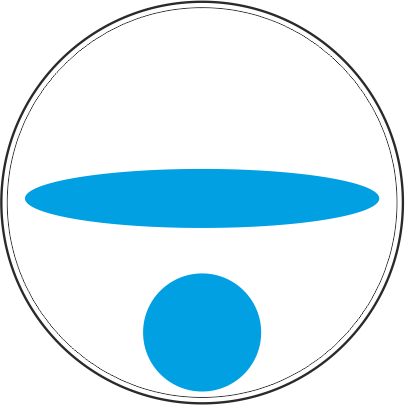
\includegraphics[width=0.3\linewidth]{../../latticeAnalyser/singleDipole.png}
			\end{center}
		\caption[Final Pattern]{Final Pattern}
		\label{singleDipole}
		\end{figure}

		\begin{figure}[bth]
			\begin{center}
				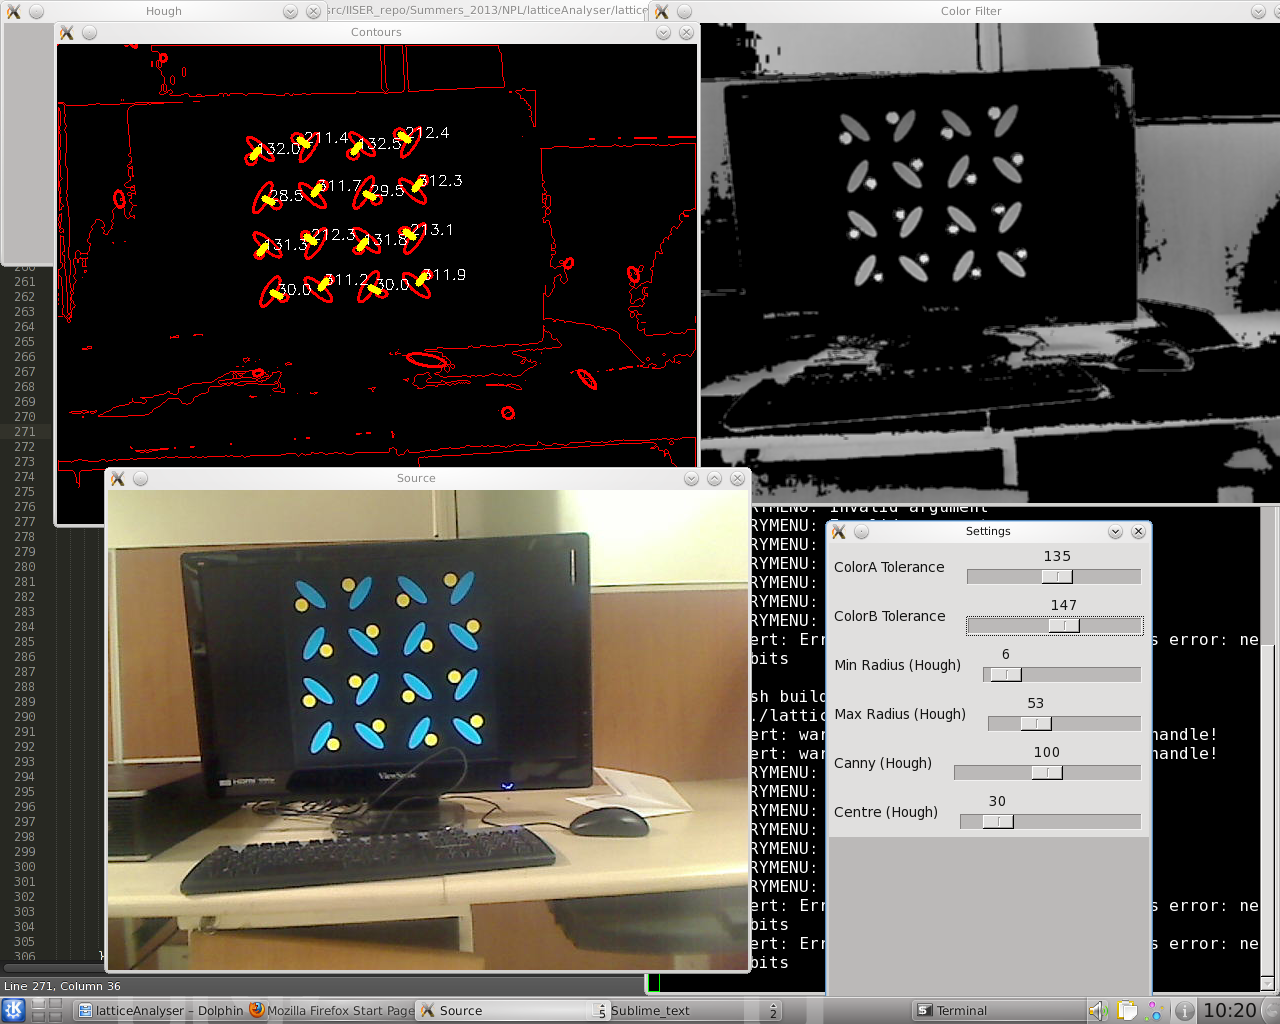
\includegraphics[width=1.1\linewidth]{../../latticeAnalyser/snapshot5.png}
			\end{center}
		\caption[Multi Shape, Single Colour]{Multi Shape, Single Colour}
		\label{snapshot5}
		\end{figure}

		After the detection, according the plan, two colours were to be used for the ellipses. However, running the hough transform twice would've dropped the detection speed to half, which wasn't worth it. It was then decided that the shapes should be made different instead of relying on two colours for the same information. After looking at various combinations, \autoref{singleDipole} was finalized, with an ellipse at the centre, and a circle along the minor axis for breaking the symmetry. This method did infact work as shown in \autoref{snapshot5}.
		\par

		\begin{figure}[bth]
			\begin{center}
				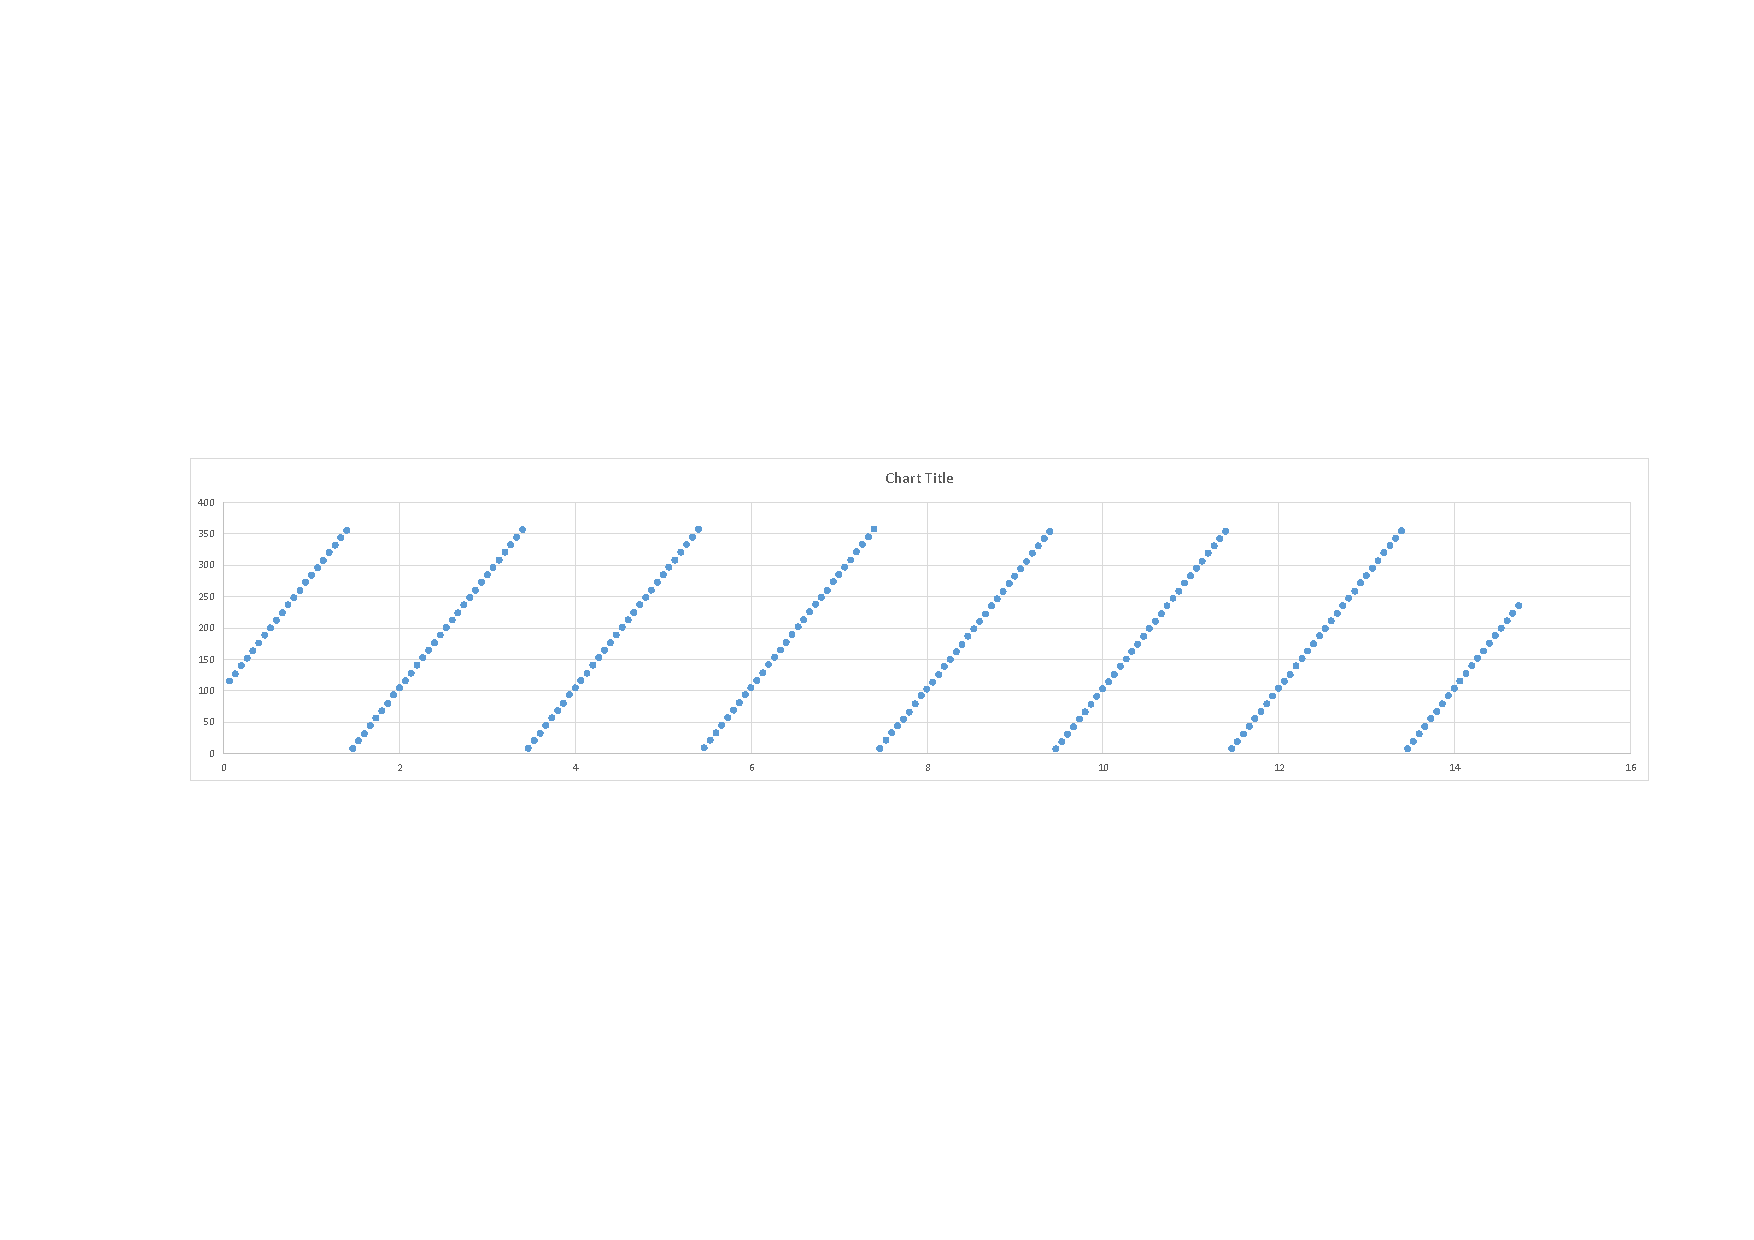
\includegraphics[width=1.1\linewidth]{../../latticeAnalyser/testGraphs}
			\end{center}
		\caption[First Observation]{First Observation}
		\label{testGraphs}
		\end{figure}

		The next challenge was to realize that a dipole detection can be missed and therefore mess up the counting, if that is the only way of uniquely identifying them. Unique identification is obviously required, as the external hardware must fire the coils of the right dipole. Thus a reference frame was used to uniquely identify the dipoles initially. This is expected to happen when they are stationary to get a good reading. In each frame, whenever a dipole is detected, it is associated with the dipole in the reference frame, by matching its location. If a dipole is not detected in a given frame, the software knows it was unable to record it and doesn't mess up neither the numbering nor the observations.
		\par

		\begin{figure}[bth]
			\begin{center}
				
\includegraphics[width=0.7\linewidth]{../../latticeAnalyser/ellipseCircleDipoles4x4_black.jpg}
			\end{center}
		\caption[Final Test Pattern]{Final Test Pattern}
		\label{testPattern}
		\end{figure}

		After implementation of the last part, an animation sequence was created in Power Point, with the dipoles rotating with a constant speed and the camera was aimed at the screen. A still from the same is given in \autoref{testPattern}. \autoref{testGraphs}, shows the angular position versus time plot, for the first dipole and yes, it is linear, just as expected. Standard deviation tests are still to be done.
		\par
		Following is the source code of the same, which has been made available online.
		\lstinputlisting[language=C++,title=latticeAnalyser.cpp]{../../latticeAnalyser/latticeAnalyser.cpp}
		
